\documentclass{article}
\usepackage[round]{natbib}
\usepackage[utf8]{inputenc}
\usepackage{graphicx}
\usepackage{authblk}

\usepackage{graphicx}
\usepackage[margin=0.85in]{geometry}
\usepackage{lineno}
\usepackage{float}
\usepackage{cleveref}
\usepackage{tabularx,ragged2e}
\usepackage{url}


\newcommand{\source}[1]{\hfill Source: {#1}} %command definition for sources in figures


\title{Evaluating global air pollution models using air quality sensors onboard a carrier bicycle in the Netherlands}
\author{Meng Lu et al. }
\date{\today}

\begin{document}

\maketitle

\section{Introduction}
Chronic exposure to air pollution poses a threat to public health. World Health Organization estimated that air pollution has contributed to 7 million deaths in 2016\citep{world2018burden}. From a medical perspective, common air pollutants such as particulate matters and nitrogen oxides (NO$_2$) damage the cardiovascular and respiratory systems \citep{anderson2012clearing, pascal2009effets}. Air pollution mapping is crucial for interventions to abate exposures. Multiple factors influence the concentration of air pollution. In the Netherlands, the NO2 concentration limit set in 2017 was exceeded for several times in places with busy traffic\citep{no2}. Emissions from traffic can be direct and indirect. Atmospheric NO$_2$ is mostly an indirect secondary emission as an oxidation result of emitted NO, while the direct primary emission as NO$_2$ is minor \citep{ukno2}. Since NO$_2$is largely produced by traffic in the Netherlands, it is therefore an important local indicator of air pollution from traffic\citep{no2}.
\par
Extensive research has mapped air pollution concentration using ground monitor station observations, satellite measurements, and ancillary NO$_2$ data (commonly called predictors, including all the variables relating to the emitting and dispersing processes of NO$_2$ such as climate, land cover, traffic network)\citep{rivera2013nitrogen, park2017individual,kharol2015assessment, isiugo2018assessing}. Ground monitors can be routinely run or are project-oriented, which requires extra cost, mainly when other attributes such as temperature and wind direction are recorded \citep{hoek2008review}. In the study of exposure assessment, ground monitors network are expensive As for satellites, their coverage range is more extensive than regional monitor networks at a higher cost \citep{hoek2008review}.  Apart from satellites and ground monitors, recent studies show a rise in urban low-cost ground sensors \citep{spinelle2015field, schneider2017mapping,isiugo2018assessing}. It is superior to satellite and regular ground monitors in its fine spatial-temporal resolution. Meanwhile, the deficits of low-cost sensors are noted as well. Measurements from low cost sensors are subject to sensor drift and interference effects. Sensor drift denotes the growing bias of sensor response due to the ageing electronic-chemical cells; Interference effects generalises the sensor's response to other pollutants, gases, temperature and relative humidity, which hampers the measurement to the target pollutant \citep{van2019calibration}. For instance, an application of low-cost sensors in the Netherlands carried in Amsterdam showed a significant signal drift for two month's of observation, while its calibration with temperature and relative humidity improve its fit with ground stations \citep{mijling2018field}.
 
NO$_2$ can be modelled using dispersion models \citep{holmes2006review,health2010traffic}, statistical models \citep{chen2019comparison}, or a combination of both \citep{molter2010modelling,marshall2008within,beelen2010comparison,dijkema2010comparison, akita2014large}. Dispersion models simulate the emission, transforming, transportation, and deposition of the pollutant, but require detailed emission inventory data and are computationally intensive, scaling a dispersion model can be at a cost of computational intractability and low prediction accuracy. Statistical models utilise geospatial predictors that are related to the emission sources (e.g. road network) and dispersion processes (e.g. meteorological data) of the pollutants \citep{briggs2000regression}, which has been used to predict high-resolution NO$_2$ at various spatial scales  \citep{Hoek2008,larkin2017global}, is the focus of this study. Most of the studies focus on long-term average NO$_2$. Recently, mapping temporally resolved NO$_2$, e.g. hourly \citep{lu2020land}, has been demonstrated to be necessary for accounting human space-time activities in exposure assessment \citep{lu2019}. The hourly models of \cite{lu2020land}, based on Land Use Regression (LUR), mapped NO$_2$ at an unprecedentedly high resolution of 5 m, and obtained a high R$^2$ validating with an external dataset, however, does it mean the hourly models could capture the spatial details? This forms the first research question of this study. 

The second research question concerns the comparison and evaluation of different statistical models. Statistical-based air pollution mapping has a long history dating back to 20 years ago \cite{briggs2000regression} and a variety of models have been developed using each or a combination of geostatistical, linear regression, and more recently, machine learning models. Several studies pinpoint the strengths and constraints of various statistical models, including standard and regularised linear regression, ensemble tree-based models, transformation-based (e.g. support vector machine), artificial neural networks, in high-resolution NO$_2$ mapping \citep{chen2019comparison, kerckhoffs2019performance, adam2014spatiotemporal, DEHOOGH2014382}. Most recently, \cite{kerckhoffs2019performance} modelling UFP (Ultra Fine Particles) obtained similar cross-validation accuracy of various statistical algorithms. \cite{chen2019comparison} modelled NO$_2$ of several European countries obtained similar cross-validation accuracy across various ensemble tree-based and linear regression models. Based on the cross-validation accuracy comparison result, \cite{chen2019comparison} and \cite{kerckhoffs2019performance} concluded on the similar performance of different statistical algorithms in modeling the spatial variation. However, neither of these two studies showed or analysed the prediction patterns. In the global NO$_2$ modeling study of Lu2020, it is found that various ensemble tree-based methods obtained almost the same cross-validation accuracy can give very different prediction patterns. This forms the second research question: to what extent can the cross-validation prediction accuracy indicate the spatial variation modelled? 

This study answers the two research questions using NO$_2$ concentrations monitored from a mobile air quality station on board a cargo bike (called “cargo-bike”) to re-evaluate temporally resolved NO$_2$  models based on different statistical algorithms. Specifically, we focused on comparing three methods, XGBoost \citep[XGB,][]{xgboost}, Random Forest \citep[RF,][]{breiman2001random} and Lasso. These methods are selected as they are representative to the current spatial prediction techniques, the implications can be generalised to comparing more methods.   %and to imply a validation method that accounts for spatial prediction patterns.  
The cargo-bike covered a selected area close to the routes followed by the Four Days Marches in Nijmegen, the Netherlands, from July 16 to 19, 2019. The cargo-bike measures NO$_2$ every morning from 8 am to 11 am, the route is repeated daily during the event. In addition, we compared the global air pollution model, which is made for 2017 and available for the daytime  (7 am – 10 pm local time), with the cargo-bike measurements to understand the amount of spatial variability that an annual global model could explain at the local time.  

\section{Data }

\subsection{Cargo-bike measurements}
The cargo-bike and the instruments on board weights 160 kg. It carries a 150 WP solar panel and can work 3 – 5 hours continuously. [detailed description to be added by Cjestmir].

The cargo-bike sensored NO$_2$ averaged over the four days have the mean of 11.21 $\mu g/m^3$. 

\begin{figure}[H]
    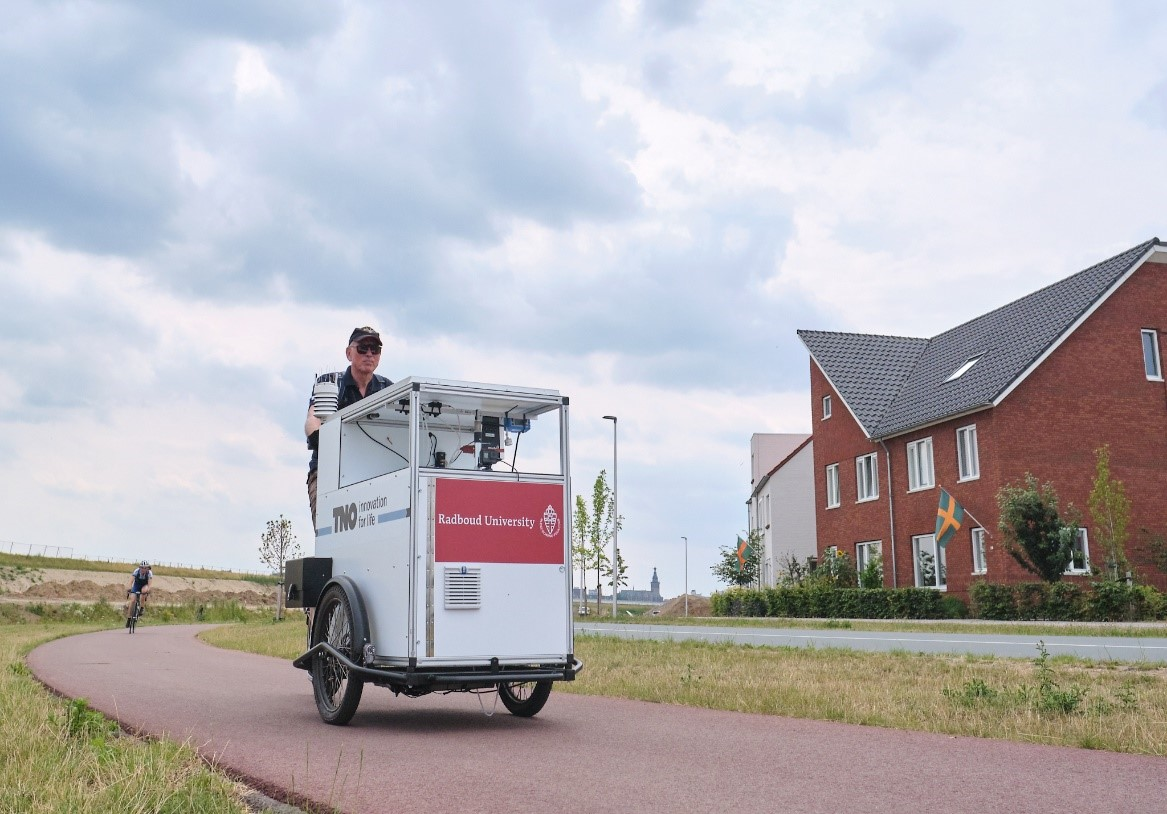
\includegraphics[width=\linewidth]{f1a.jpg}
    \label{bike}
    \caption {bikefits}
\end{figure}
\begin{figure}
    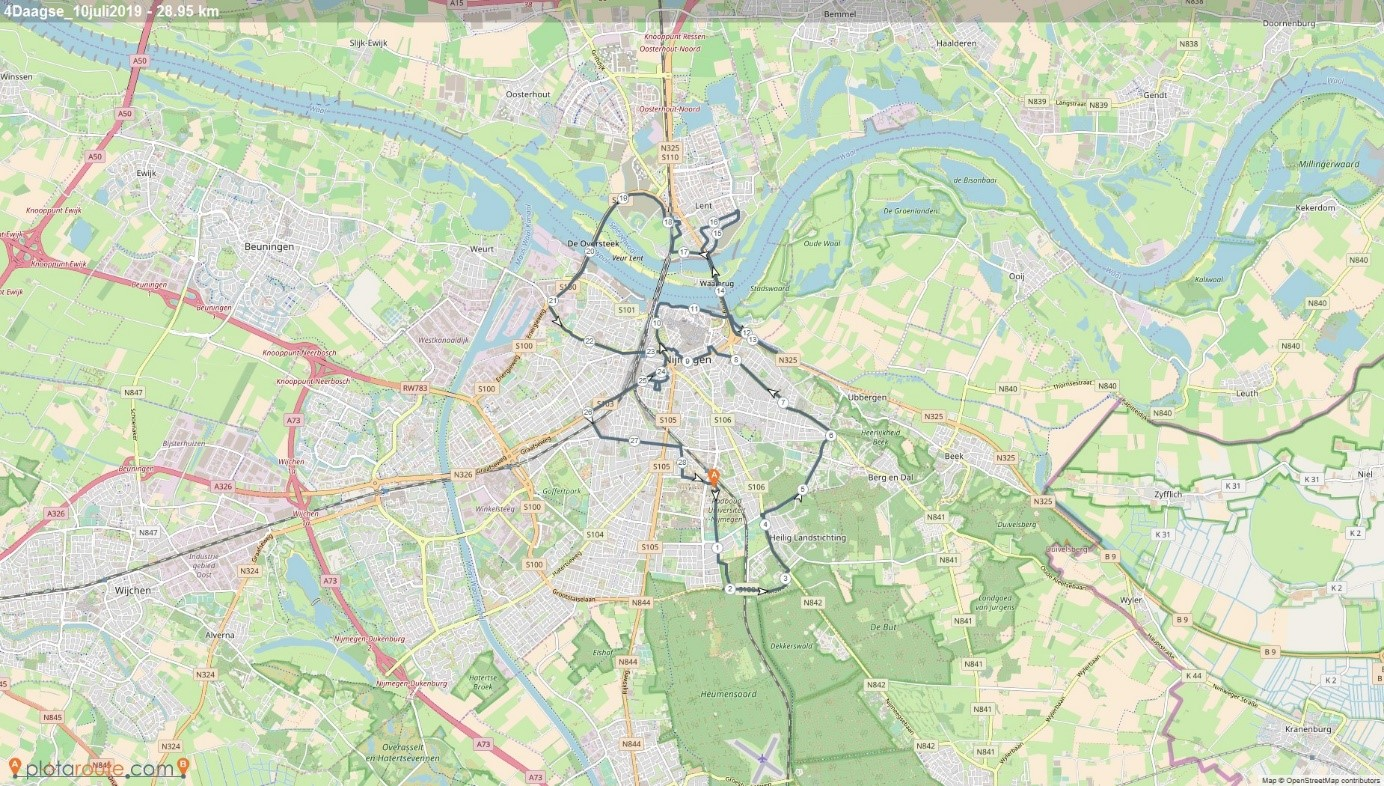
\includegraphics[width=\linewidth]{f1b.jpg}
    \label{route}
    \caption {routes taken by the cargo-bike on openstreetmap\citep{openstreetmap}.}
\end{figure}
%“A” indicates the starting point.The point numbers indicated on the map are used to indicate the routes. For example route from point 1 to point 2, which is called route 1-2 in this study.

\subsection{Ground monitor stations in Netherlands and Germany}

Since the Netherlands (41,543 $km^2$) contains only 77 stations, we also incorporated the ground monitor network from Germany (357.386 $km^2$) to improve the modelling accuracy. The ground monitoring stations data are from European Environment Agency (cite) for the Netherlands and the Umwelt Bundesamt (cite) for Germany. Stations with inadequate data such as missing value at certain hours are neglected. The measurements are downloaded the same days as the Cargo-bike measurements and from 7:00 am - 11:59 am. This dataset is called NLDE.

\subsection{Ground monitor stations in Nijmegen}
The ground measurements are gathered from two LML stations, one is the Nijmegen-Graafseweg station (called Graafseweg station, Latitude: 51.941372, Longitude 5.857777). The other is Nijmegen-Ruyterstraat station (called Ruyterstraat station, Latitude: 51.838221, Longitude: 5. 856938). The station is managed by RIVM to monitor air pollution from local traffic. The measurements averaged over the same periods of cargo-bike is 23.25 ug/m3 at Graafseweg and 14.03 ug/m3 at Ruyterstraat.
 

 
\subsection{Geospatial predictors}
 The geospatial predictors were calculated at 25 m resolution. They are either spatial attributes aggregated within a circular ring centred at each sensor or prediction location, called buffered predictors, or values of the spatial attribute at the observation or prediction location. The buffered predictors include industry areas, roads, and population. Gridded variables include wind speed, temperature, elevation, and satellite products from TROPOMI, OMI, and a GEOS-CHEM \citep{bey2001global,GEOS-CHEM} annual NO$_2$ surface concentration product \citep{geddes2016long}. The predictors used in this study are the same as lu2020, which provide detailed description of the predictors . 
  

\section{Methods}
The NEDL data are aggregated in two ways, one is the mean of all hours and days, called NEDL-avg dataset, and the other the mean of each hour of the days corresponding to the time of cargo-bike measurements, called NEDL-hr dataset. The data exploration and XGB and RF hyperparameter optimisation are based on NEDL-avg. NEDL-hr is mainly used in the modelling process . 

\subsection{Spatial stationarity and dependency}
We used GWR(Geographically Weighted Regression) to explore local stationarity of the NLDE dataset (supplement). Variograms with various cut-offs are used to inspect spatial correlations (supplement). No significant location variability is found from errors, weights, and R$^2$ of GWR. No spatial correlation is found among the station measurements.     

\subsection{RF and XGB hyperparameter optimization}
The NLDE-avg dataset is used for hyperparameter optimization, through grid search, with 5-fold cross-validation. For XGB, the learning rate (eta), number of iterations (rounds), maximum tree depth (max.tree.depth) and gamma are tuned, each time 70\% of data is drawn from the training set. At last, the optimal set of hyperparameters are eta = 0.05, rounds = 200, max.tree.depth = 3, gamma = 1. For random forest, the minimum number of trees on the end nodes (min.node.size), and  number of variables that are randomly draw for each tree (mtry) are tunned. The optimal setting is min.node.size = 5 and mtry =12, the number of trees is set to 1000 for random forest, which is a relatively high value, but is a safe choice as the high number of trees will not negatively affect model performance.

\subsection{Separating between background and traffic areas}
To validate the predictions close to roads and faraway from roads, we made two groups. If the location is within 500 m distance away from the primary roads, they are grouped into traffic areas, if the location is farther away from the primary roads, they are grouped into background areas. Figure X shows the cargo-bike routes that are in traffic areas and background areas. 
separating between traffic and background areas, cargo-bike measurements.
\begin{figure}[H]
    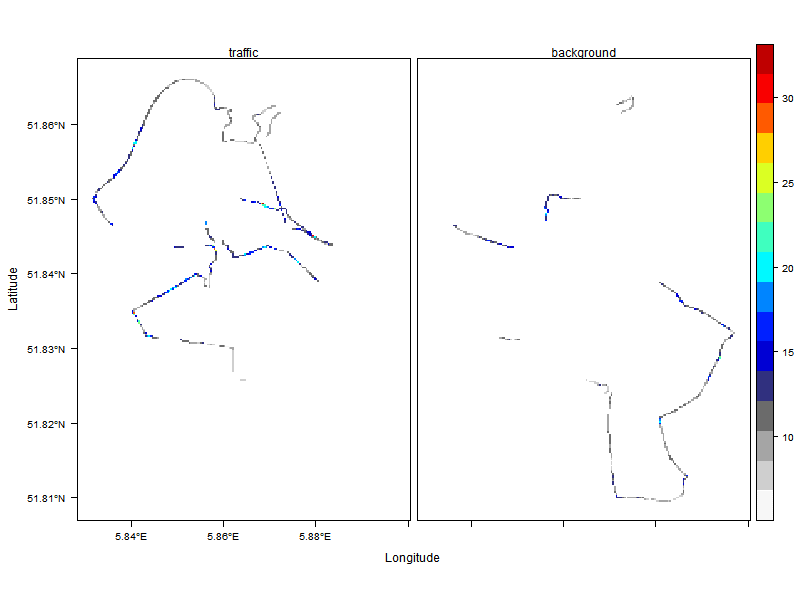
\includegraphics[width=\linewidth]{f2.png}
    \label{seperate}
    \caption {separating between traffic and background areas, cargo-bike measurements.}
\end{figure}

  \subsection{Global NO$_2$ model predictions}
%The openaq data is used for the global model predictions (see Lu et al. 2020). Three methods are evaluated in this study, namely xgboost, random forest, and Lasso. Based on hyperparameter setting recommendations provided by Lu et al (2020) We used 1000 trees for all the methods. The maximum tree depth for xgboost is set to 6 and learning rate set to 0.02. Other settings are the same as Lu2020. 
As the global model predictions are for entire year, we scale them to the same time-span as the cargo-bike measurements by multiplying the predictions to the ratio between the global model prediction and the LML measurements averaged over the timespan of the cargo-bike measurements (July 16 -19, 8 am - 11 am), which means after scaling, the mean of the xgboost, random forest, and Lasso predictions are also 23.25 ug/m3 if scaled using the Graafseweg station and 14.03 if scaled using the Ruyterstraat station.   

\section{Result}
\subsection{Variable importance}

\begin{table}[H] \centering 
  \caption{Ranking of the top 20 important variables of XGBoost and Random Forest, for the local model} 
    \label{nlde_vimp} 
\begin{tabular}{@{\extracolsep{5pt}} ccc} 
\\[-1.8ex]\hline 
\hline \\[-1.8ex] 
Rank & XGBoost & Random Forest \\ 
\hline \\[-1.8ex] 
1 & pop3k & pop3k \\ 
2 & road\_class\_2\_25 & road\_class\_M345\_3000 \\ 
3 & road\_class\_M345\_3000 & road\_class\_M345\_5000 \\ 
4 & road\_class\_M345\_5000 & road\_class\_2\_25 \\ 
5 & road\_class\_2\_50 & road\_class\_2\_50 \\ 
6 & road\_class\_1\_5000 & pop5k \\ 
7 & temperature\_2m\_6 & road\_class\_2\_100 \\ 
8 & wind\_speed\_10m\_9 & elevation \\ 
9 & wind\_speed\_10m\_4 & pop1k \\ 
10 & road\_class\_M345\_50 & wind\_speed\_10m\_9 \\ 
11 & road\_class\_M345\_100 & road\_class\_1\_5000 \\ 
12 & pop1k & temperature\_2m\_6 \\ 
13 & road\_class\_M345\_300 & wind\_speed\_10m\_10 \\ 
14 & road\_class\_M345\_25 & wind\_speed\_10m\_4 \\ 
15 & elevation & road\_class\_M345\_100 \\ 
16 & wind\_speed\_10m\_10 & wind\_speed\_10m\_6 \\ 
17 & trop\_mean\_filt & trop\_mean\_filt \\ 
18 & pop5k & road\_class\_M345\_300 \\ 
19 & temperature\_2m\_5 & wind\_speed\_10m\_2 \\ 
20 & road\_class\_1\_1000 & wind\_speed\_10m\_8 \\ 
\hline \\[-1.8ex] 
\end{tabular} 
\end{table} 

\begin{table}[H] \centering 
  \caption{cross validation results of the NLDE-XGB, NLDE-RF, NLDE-Lasso models, $\mu g/m^3$} 
    \label{nlde_vimp} 
\begin{tabular}{@{\extracolsep{5pt}} cccccccc} 
\\[-1.8ex]\hline 
\hline \\[-1.8ex] 
 
&RMSE & RRMSE & IQR & rIQR & MAE & rMAE & rsq \\\hline \\[-1.8ex] 
 
XGB	&7.36 	& 0.36 &	6.54 &	0.37 &	5.09& 	0.25 &	0.71\\
RF	&7.36	& 0.36 &	6.42 &	0.36 &	5.04&	0.25 &	0.70 \\
Lasso &	8.51 &	0.42 & 8.67	& 0.49	&6.20 &	0.31	&0.61\\
\hline \\[-1.8ex] 
\end{tabular} 
\end{table} 

\begin{figure}[H]
    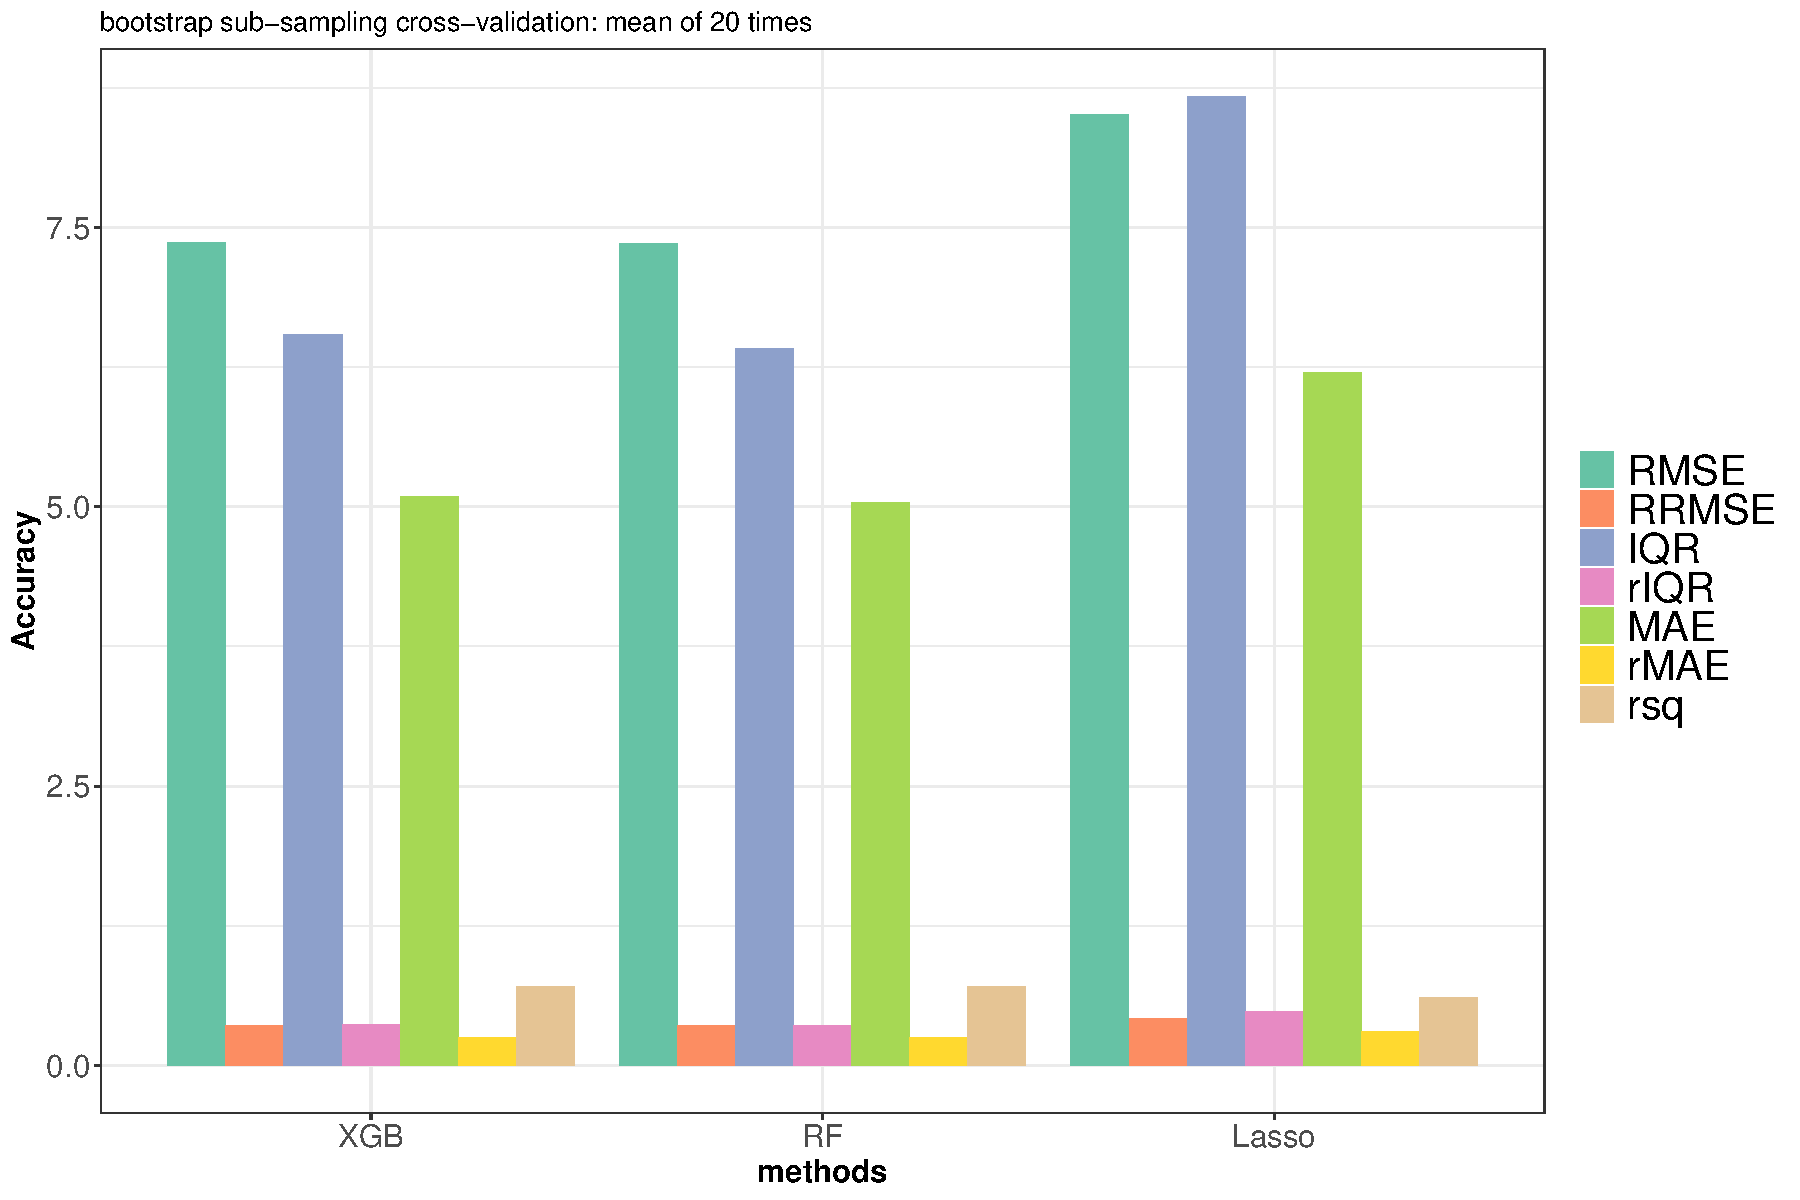
\includegraphics[width=\linewidth]{w1-1.pdf}
    \label{accuracy}
    \caption { Accuracy assessed for NLDE-XGB, NLDE-RF, NLDE-Lasso.}
  \end{figure}
  
\begin{figure}[H]
    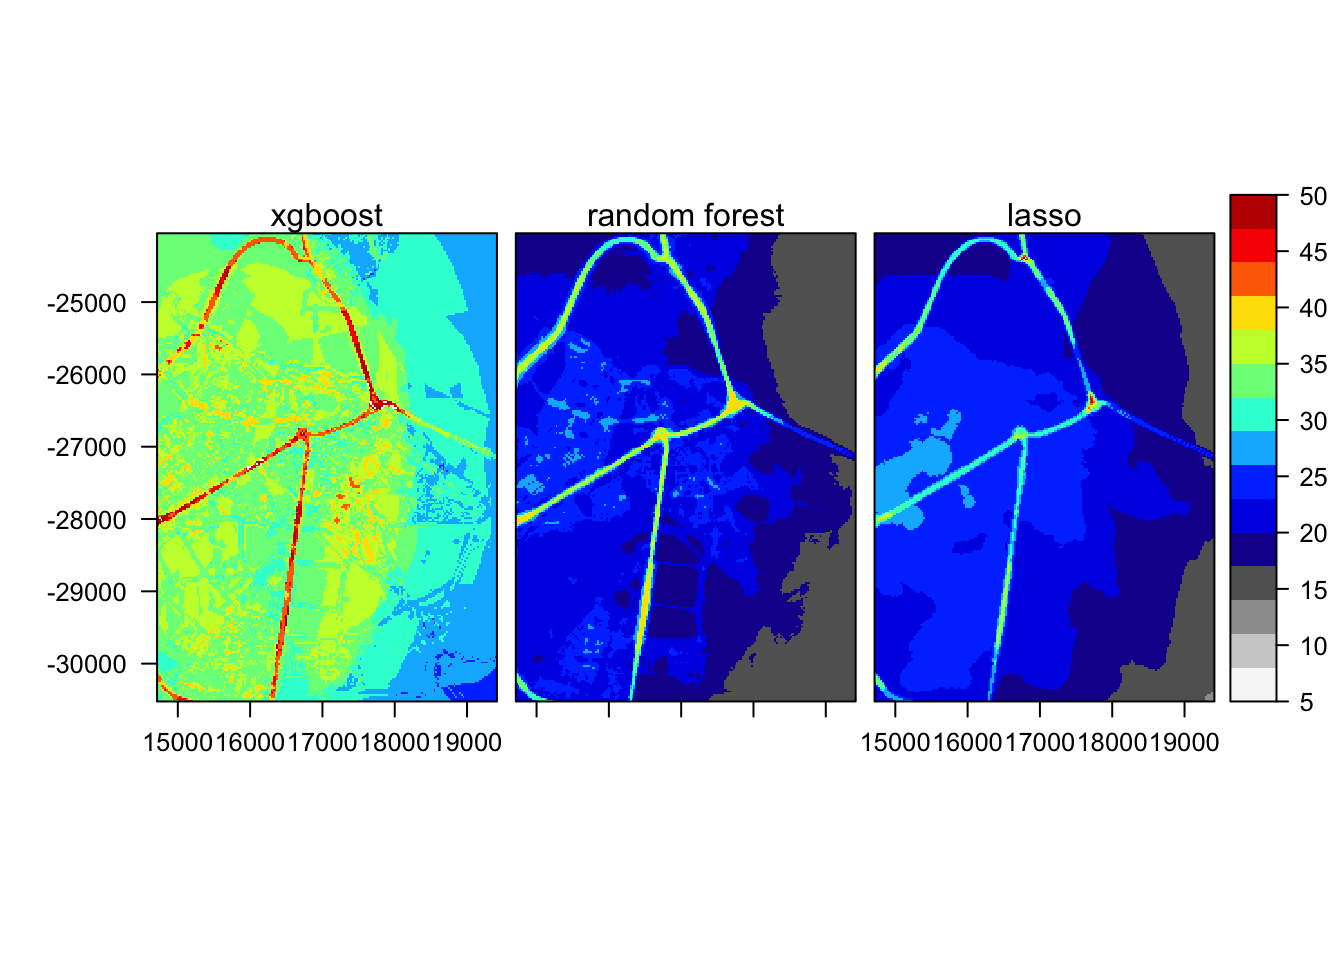
\includegraphics[width=\linewidth]{NLDE.png}
    \label{nldepred}
    \caption {predictions from NLDE-XGB, NLDE-RF, NLDE-Lasso.}
\end{figure}
\begin{figure}[H]
    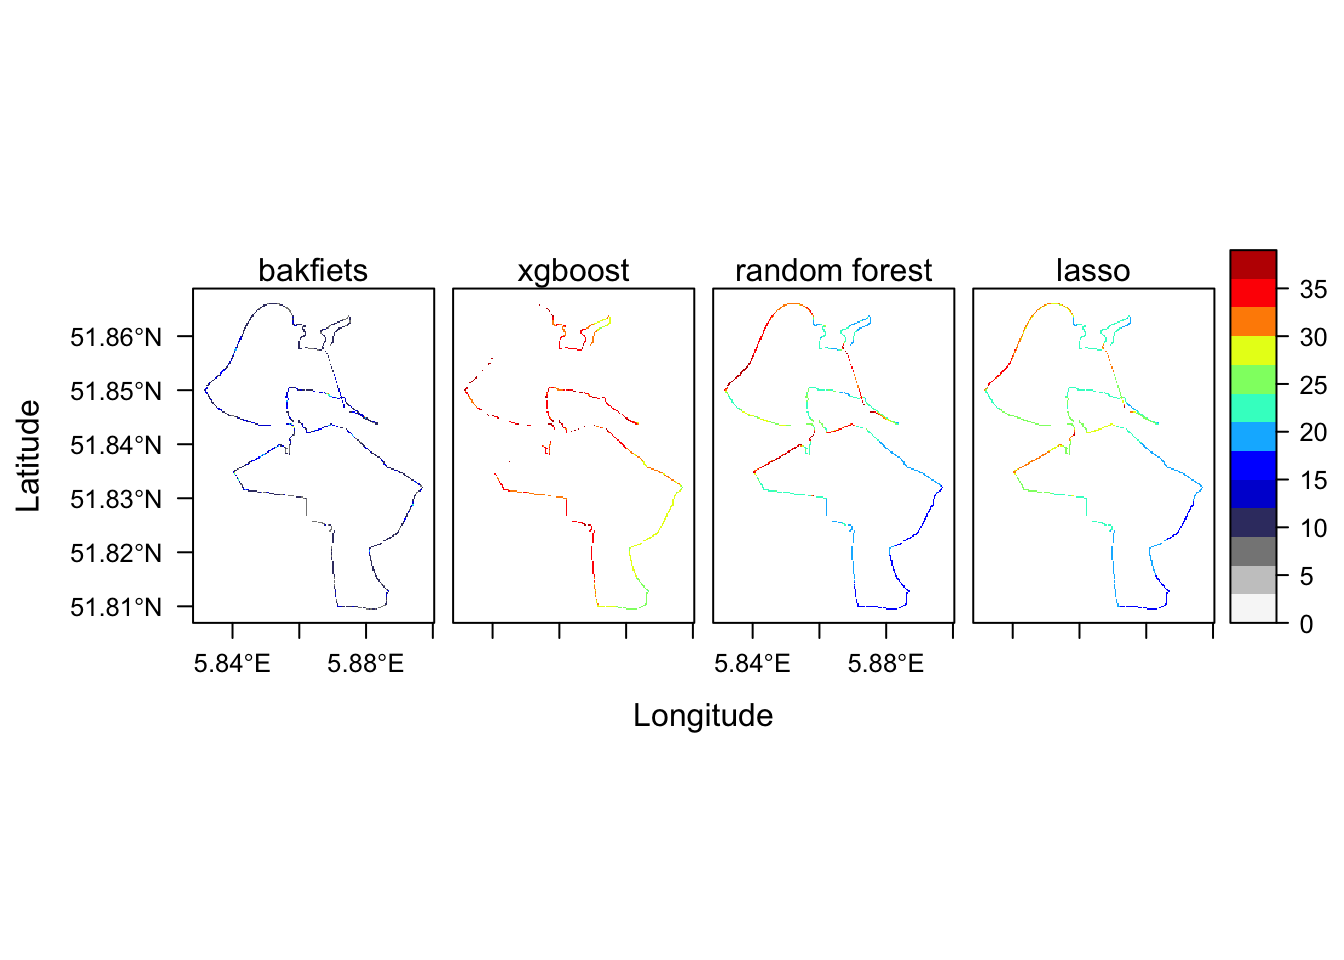
\includegraphics [scale = 0.3 ]{NLDEtrack.png}
    \label{nldevsbak}
    \caption { NLDE model predictions and cargo-bike measurements}
\end{figure}

\subsection{Compare with bakfiets measurements}
The Pearson's correlation between NLDE- XGB, NLDE-RF, NLDE- LA  and Bakfiets measurements are respectively 0.24, 0.28, 0.23. The median differences are respectively 34, 23, 23 $\mu g/m^3$. 

 
%pearson correlation coefficient`
 %         xgbnij    rfmnij    Lamnij
%xgbnij 1.0000000 0.7956444 0.7786702
%rfmnij 0.7956444 1.0000000 0.9287154
%Lamnij 0.7786702 0.9287154 1.0000000

%mean
%  xgbnij   rfmnij   Lamnij 
%32.99156 20.67016 21.43969 

\subsection{Global model predictions}
The mean of xgboost, random forest, and Lasso predictions over the area of Nijmegen (called predictions) are respectively 25.77, 22.38, and 26.54 ug/m3. The Nijmegen predictions are shown in figure X. From the figures, the xgboost and random forest predictions reveal more details, they also obtained a higher prediction accuracy (see the global paper) compared to Lasso. Comparing the figure X with the predictors (supplement figure SF2), it can be observed that the predictions reveal primary road patterns. The paired Pearson correlation between three Nijmegen predictions in are: 0.8 for random forest vs. Lasso, 0.81 for random forest vs. xgboost, and 0.94 for Lasso vs. random forest.
\begin{figure}[h!]
    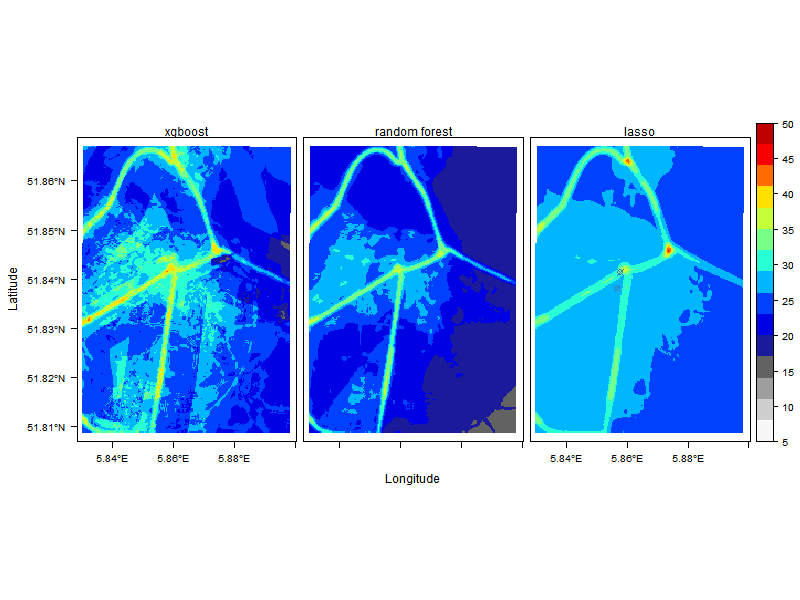
\includegraphics[width=\linewidth]{f3.png}
    \label{seperate}
    \caption {predictions from three global models: xgboost, random forest and lasso. The LML stations that are used in the global model are shown in the Lasso prediction plot.}
\end{figure}
\subsection{Validation with Cargo-bike measurements}

\begin{figure}[H]
    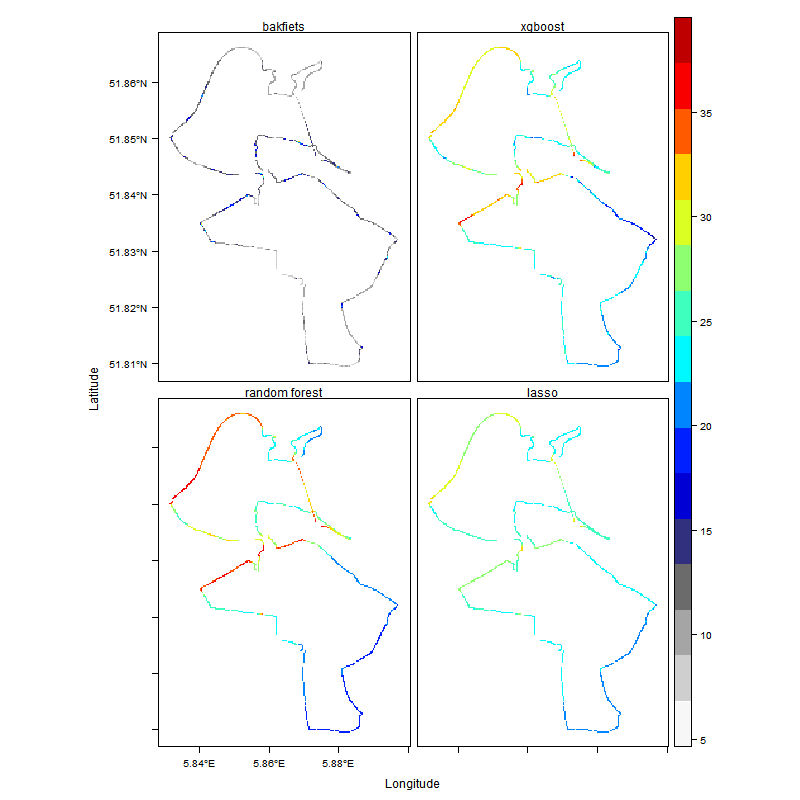
\includegraphics[width=\linewidth]{f4.png}
    \label{seperate}
    \caption {Averaged cargo-bike measurements and global model predictions (scaled). a: scale the cargo-bike using the Graafseweg LML station.}
\end{figure}
The cargo-bike measurements (the distribution is shown in supplementary figure SF1) show higher NO$_2$ in the west and middle, from points 19 -21, 24 -25, and around point 9 (figure 1, called route 19-21, 24-25, and 9), which align well with predictions from the three global models. However, the spatial variations of the cargo-bike measurements are much smaller compared to the global model predictions. The route 19-21 and route 24-25 are estimated much higher by the global models, most notably random forest.    
 
Figure X shows averaged cargo-bike measurements and scaled global model predictions at the cargo-bike track. It shows the global model predictions are higher in magnitudes, however, remember the mean of the global model prediction is closer to the mean of the LML ground station measurements. 
\begin{figure}[H]
    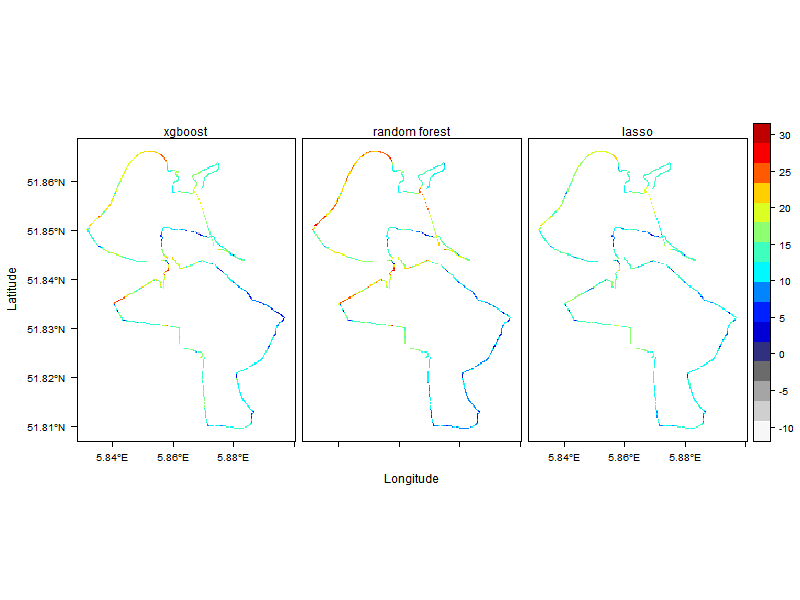
\includegraphics[width=\linewidth]{f4a.png}
    \label{Graafseweg}
    \caption {scale the cargo-bike using the Graafseweg station. The differences between scaled global model predictions and cargo-bike meausrements, the values are the subtraction of cargo-bike measurements from global model predictions (model prediction - bike measurements), in ug/m3.}
\end{figure}
\begin{figure}[H]
    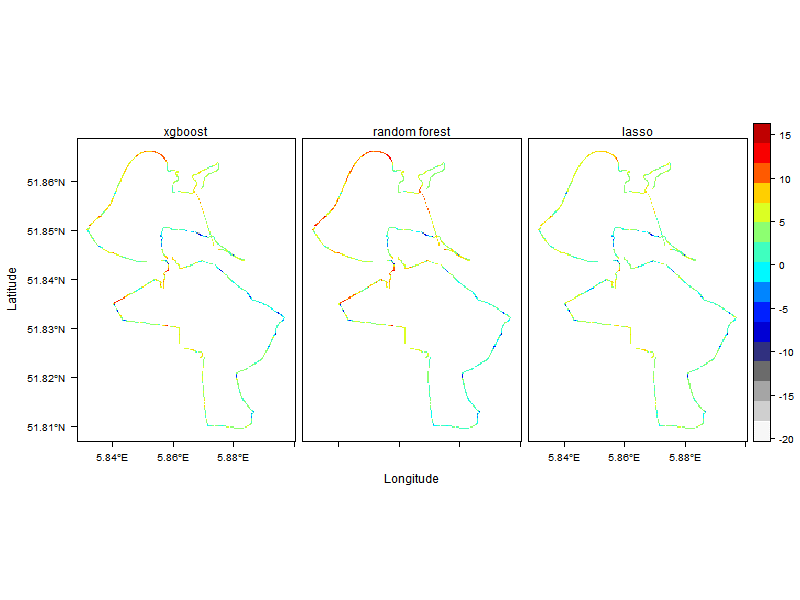
\includegraphics[width=\linewidth]{f4b.png}
    \label{ruyterstraat}
    \caption {scale the cargo-bike using the ruyterstraat station.}
\end{figure}

\section{Discussion}
\newpage
\bibliographystyle{plainnat}
\bibliography{ref}

\end{document}

https://www.umweltbundesamt.de/en
http://discomap.eea.europa.eu/Index/
